\documentclass{article}
\usepackage[utf8]{inputenc}
\usepackage{cmap}					% поиск в PDF
\usepackage{mathtext} 				% русские буквы в формулах
\usepackage[T2A]{fontenc}			% кодировка
\usepackage[utf8]{inputenc}			% кодировка исходного текста
\usepackage[english,russian]{babel}	% локализация и переносы
\usepackage{indentfirst}
\usepackage{graphicx}
\graphicspath{ {./images/} }
\usepackage{xcolor}
\usepackage{color}
\title{Отчёт по 7 лабе}
\date{October 2022}

\begin{document}

\maketitle

\section{Выбранный инструмент}
\section{Вид проекта}
\section{Программа}
\section{Тесты}
\section{Результаты}

\newpage
\huge {Выбранный инструмент} \\ \\
\large {\textbf{IntelliJ IDEA} — интегрированная среда разработки программного обеспечения для многих языков программирования, в частности Java, с широким набором интегрированных инструментов для рефакторинга, которые позволяли программистам быстро реорганизовывать исходные тексты программ. Дизайн среды ориентирован на продуктивность работы программистов, позволяя сконцентрироваться на функциональных задачах, в то время как IntelliJ IDEA берёт на себя выполнение рутинных операций. Среди прочих возможностей, среда хорошо совместима со многими популярными свободными инструментами разработчиков, такими как CVS, Subversion, Apache Ant, Maven и JUnit}
\\ \\
\large{\textbf{Apache Maven} — фреймворк для автоматизации сборки проектов на основе описания их структуры в файлах на языке POM, являющемся подмножеством XML}
\\ \\
\large{\textbf{JUnit} — фреймворк для модульного тестирования программного обеспечения на языке Java.}

\newpage
\huge{Вид проекта} \\ \\
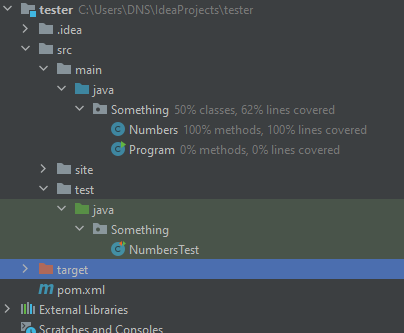
\includegraphics[scale=1]{tester.png}

    \large{файлы проекта}
\\ \\
\large{Папка Java (\textcolor{blue}{синяя}) - источники. В ней хранится метод и main файл(Program) }
\\ \\
\large{Папка Java (\textcolor{green}{зелёная}) - тесты. В файле NumbersTest хранятся все написанные тесты, и можно проверить как один тест, так и все сразу}
\\ \\
\large{\textbf{pom.xml} - это XML-файл, который содержит информацию о конфигурации и деталях проекта, используемых при создании проекта на Maven. Он всегда находится в базовом каталоге проекта. Этот файл также содержит описание задач, список и параметры плагинов.}

\newpage
\huge{Программа} \\ \\
\large{\textcolor{blue}{\textbf{''}} Папка Java (\textcolor{blue}{синяя}) - источники. В ней хранится метод и main файл(Program)\textcolor{blue}{\textbf{''}}}
\\ \\
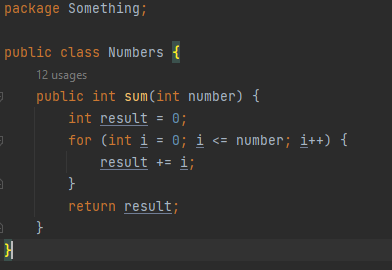
\includegraphics[scale=1]{Numbers.png}

Метод Numbers - считает сумму чисел от 1 до введённого числа
\\ \\
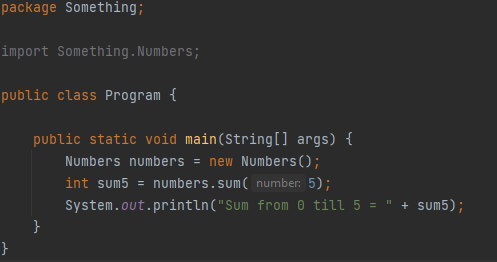
\includegraphics[scale=1]{Program.png}

Program - для проверки работы метода
\\
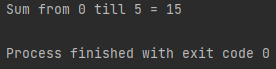
\includegraphics[scale=1.5]{nice.png}

\newpage
\huge{Тесты} \\ \\
\Large{Всего тестов получилось 11}
\\ \\
\Large{\textbf{Test1}}
\\ \\
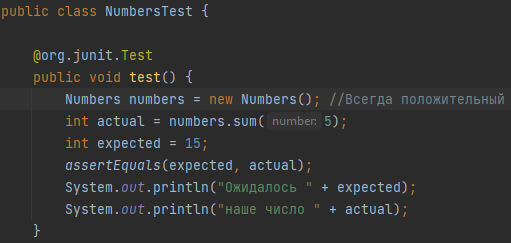
\includegraphics[scale=1]{Test1.png}
\\ \\
\Large{\textbf{Test2}}
\\ \\
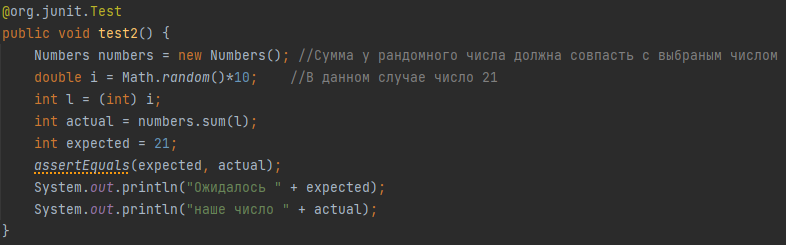
\includegraphics[scale=0.8]{Test2.png}
\\ \\
\newpage
\Large{\textbf{Test3}}
\\ \\
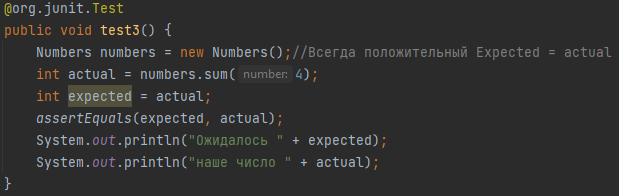
\includegraphics[scale=1]{Test3.png}
\\ \\
\Large{\textbf{Test4}}
\\ \\
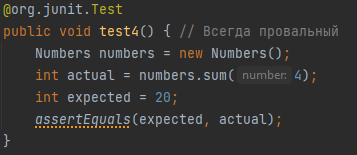
\includegraphics[scale=1]{Test4.png}
\\ \\
\Large{\textbf{Test5}}
\\ \\
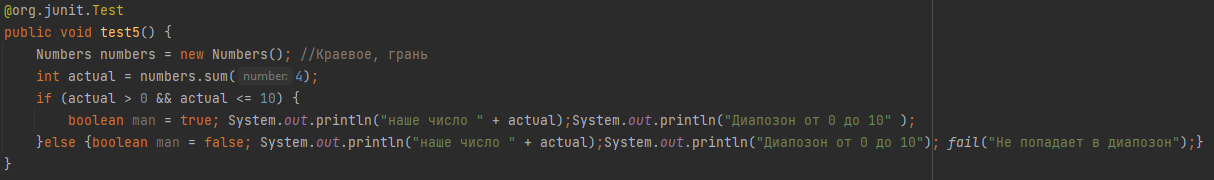
\includegraphics[scale=0.5]{Test5.png}
\\ \\
\newpage
\Large{\textbf{Test6}}
\\ \\
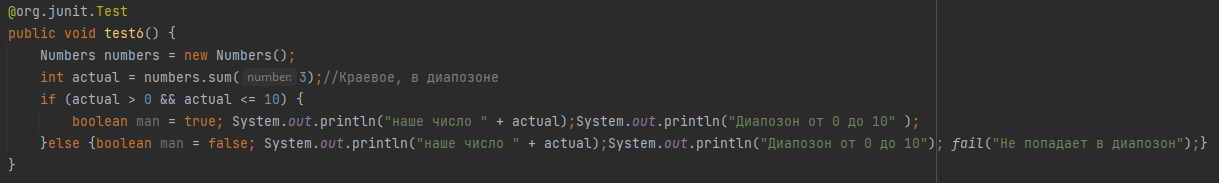
\includegraphics[scale=0.5]{Test6.png}
\\ \\
\Large{\textbf{Test7}}
\\ \\
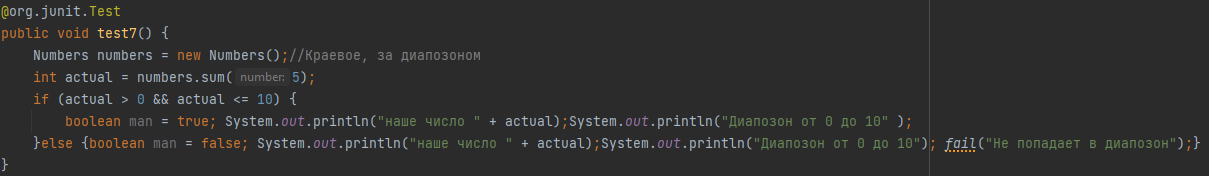
\includegraphics[scale=0.5]{Test7.png}
\\ \\
\Large{\textbf{Test8}}
\\ \\
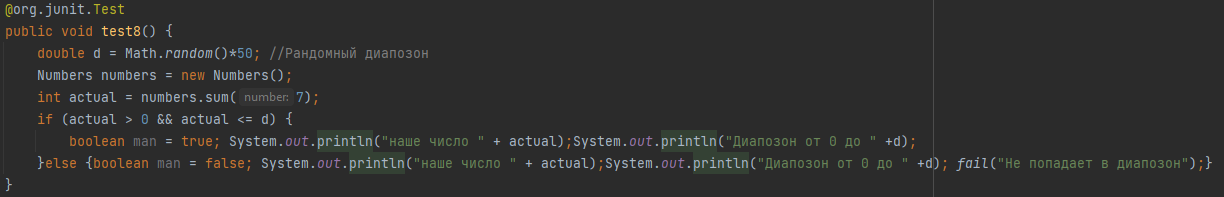
\includegraphics[scale=0.5]{Test8.png}
\\ \\
\newpage
\Large{\textbf{Test9}}
\\ \\
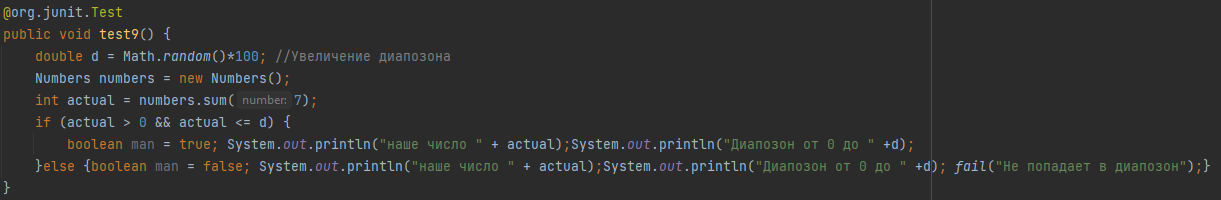
\includegraphics[scale=0.5]{Test9.png}
\\ \\
\Large{\textbf{Test10}}
\\ \\
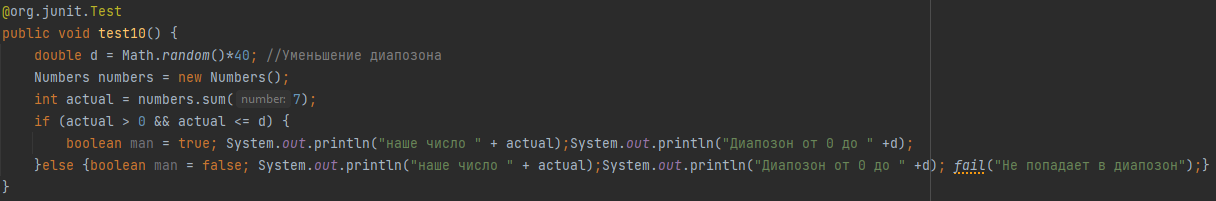
\includegraphics[scale=0.5]{Test10.png}
\\ \\
\Large{\textbf{Test11}}
\\ \\
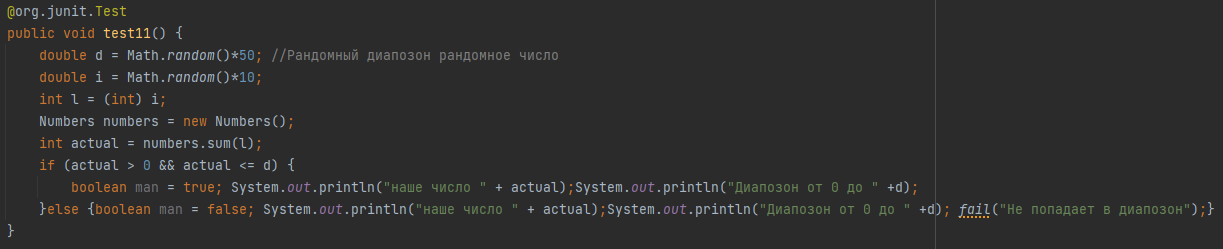
\includegraphics[scale=0.5]{Test11.png}

\newpage
\huge{Результаты} \\ \\
\Large{Результат тестов можно узнать как у одного конкретного теста, так и у всех одновременно}
\\ \\
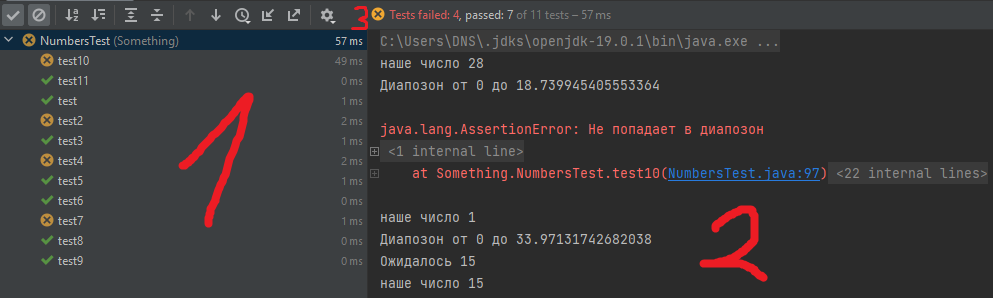
\includegraphics[scale=0.8]{Screenshot_3.png}

\Large{Результат всех тестов}
\\ \\
1 - Кратко результаты тестирования, графически. \\ Можно кликнуть на каждый тест и посмотреть результ
\\ \\
2 - Конкретные результаты тестирования. Можно видеть почему тест пройден или не пройден
\\ \\
3 - Краткие результаты тестирования/Статистика пройденных и не пройденных тестов
\newpage
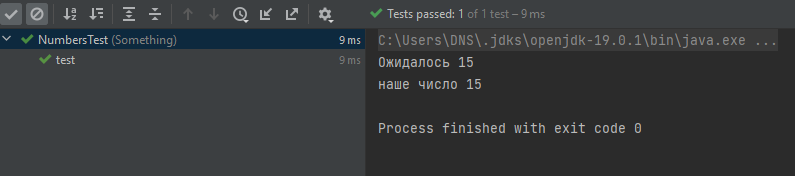
\includegraphics[scale=0.8]{один тест.png}
\Large{Результат одного теста}
\\ \\
Также есть тесты которые требуют множественного вызова, т.к. данные в них берутся рандомные, к ним относятся тесты 2, 8, 9, 10, 11
\\
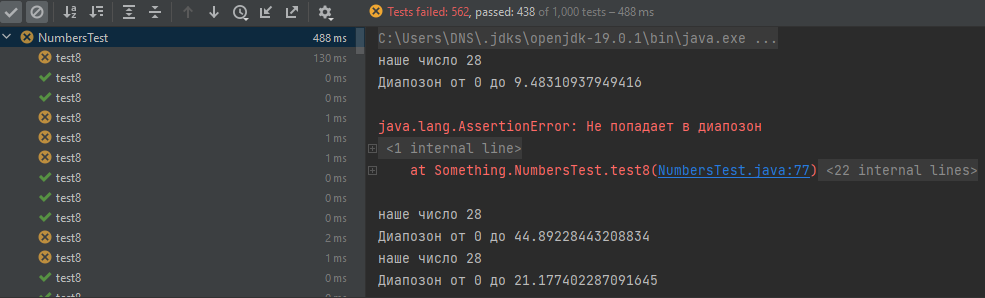
\includegraphics[scale=0.8]{тест 8 2.png}
Пример вызова 1000 раз теста номер 8
\\ \\ Здесь нас будут интересовать статистические данные, а именно то что 562 теста не прошло тестирование и 438 прошло, из этого можно выявить примерный процент для прохождения теста
\\ \\
\newpage
\Huge{\textbf{Шансы прохождения для тестов:}}
\begin{enumerate}
    \item 100\%
    \item 9,1\%
    \item 100\%
    \item 0\%
    \item 100\%
    \item 100\%
    \item 0\%
    \item 43,8\%
    \item 71,8\%
    \item 32,2\%
    \item 56,9\%
\end{enumerate}
\end{document}
